% ================================================================= 1
\section{Introduction}
An agent's long-term memory is a stream of small decisions. Is this statement new? Does it replace an older one? Is
``Priya'' the Priya we already know? Is this fact worth a place in the context window? Most memory systems have a
generative LLM write these decisions as text (Mem0's \code{ADD}/\code{UPDATE}/\code{DELETE}~\cite{mem0}, Graphiti's
edge invalidation~\cite{zep}), so the surrounding code gets no probability to act on: it cannot say ``act only when
sure'' or treat a destructive decision more cautiously than a harmless one.

\mx{} (package \code{memx}) splits the work. A generative model (Claude Haiku) turns text into candidate facts.
\textbf{Jev}, TypeSafe's calibrated decision model~\cite{typesafe}, makes every decision about them and returns a
probability for each option; code applies the thresholds and logs every answer. Jev is not new to memory
(Section~\ref{sec:related}); \mx{}'s contributions are the policies around it:
\begin{enumerate}
\item \textbf{Scope-local corrections.} Scopes are dot paths (\code{memory.acme.alex.agent1}); reads inherit from
ancestors. A model-judged correction in a narrow scope \emph{shadows} the broader fact for that branch only
(Section~\ref{sec:reconcile}).
\item \textbf{A banded, five-way reconcile verdict} (same, candidate replaces, neighbour covers, related, unrelated).
Similarity decides only whether Jev is asked; destructive verdicts need $P\ge0.9$ and pass three code guards.
\item \textbf{Asymmetric entity priors.} Different spellings merge only if Jev is sure they match; identical names split
only if Jev is sure they differ (Section~\ref{sec:entities}).
\item \textbf{Joint grading of linked facts} at recall, so a bridge fact is judged with the fact that led to it
(Section~\ref{sec:recall}).
\item \textbf{A complete decision record}: every verdict with its probabilities, so a changed policy can be re-applied
to existing memory without re-extraction (Section~\ref{sec:audit}).
\end{enumerate}

\paragraph{Results in brief} Against mem0 with extraction, embeddings, answering model and judge held equal, \mx{}
gives the answering model \textbf{2--9 times fewer memory tokens} on every benchmark, at the same ingest cost: on
LongMemEval-S, 80.5\% with 358 tokens against mem0's 76.8\% with 1,650, and 89.0\% from full memory ($p=0.013$ against
mem0); on BEAM's contradiction and update questions, 60.0\% against 53.8\% ($p=0.049$). Both memory systems beat a
full-context baseline that reads 117k tokens per question. On two-hop questions the walk turns 28 correct answers into
41. Zep's Graphiti, with its LLM judge or with Jev, scored lower at four to five times \mx{}'s ingest cost.

% ================================================================= 2
\section{Related work}\label{sec:related}

Mem0~\cite{mem0} originally let an LLM choose \code{ADD}/\code{UPDATE}/\code{DELETE}/\code{NOOP}; its current
open-source pipeline is additive and resolves contradictions at read time~\cite{mem0v3}, which is the version we
benchmark. Zep's Graphiti~\cite{zep} keeps a bi-temporal graph and invalidates contradicted edges; since October 2026 it
can route deduplication and contradiction decisions to Jev at fixed thresholds of 0.7 and 0.8~\cite{graphitijev}.
Jev-Mem~\cite{jevmem} uses Jev as the controller of a memory graph, Mnemon~\cite{mnemon} uses it to judge raw records at
read time, and a dozen open-source projects use it for write gates, injection checks, supersession, reranking and entity
resolution~\cite{jevmemoss,invalidate,dshmem,hindsightjev,supermemoryjev,slashid}. Independent studies find Jev's
choice probabilities broadly calibrated but sensitive to phrasing and prevalence~\cite{deusser,jevsurvey,meng}, which
is why \mx{} checks its own thresholds (Section~\ref{sec:decisions}). Table~\ref{tab:prior} places \mx{} among these
systems; we found no prior system with model-decided, subtree-scoped supersession, the banded five-way verdict, the
asymmetric entity priors, or the $\max(\text{alone},\text{linked})$ grading rule.

\begin{table}[!htb]
\centering\small
\setlength{\tabcolsep}{4pt}
\begin{tabularx}{\linewidth}{@{}>{\raggedright\arraybackslash}p{2.7cm} >{\centering\arraybackslash}X >{\centering\arraybackslash}X >{\centering\arraybackslash}X >{\centering\arraybackslash}X >{\centering\arraybackslash}X >{\centering\arraybackslash}X >{\centering\arraybackslash}X@{}}
\toprule
\thead{System} & \thead{Calibrated write gate} & \thead{Typed injection check} & \thead{Directional supersede} & \thead{Entity merge / split} & \thead{Joint link grading} & \thead{Scope-local correction} & \thead{Decision log}\\
\midrule
Mem0 / Mem0g (2025)~\cite{mem0} & \no & \no & \half{} LLM op & \half{} embedding & \no & \no & \half\\ \rowrule
Mem0 OSS v3~\cite{mem0v3} & \no & \no & \no{} add-only & \half & \no & \no & \half\\ \rowrule
Zep / Graphiti~\cite{zep} & \no & \no & \half{} LLM, global & \half{} LLM & \no & \no & \half\\ \rowrule
Graphiti + Jev (Oct 2026)~\cite{graphitijev} & \yes{} 2 fixed & \no & \half{} binary, global & \half{} one threshold & \no & \no & \half\\ \rowrule
Jev-Mem~\cite{jevmem} & \yes & \no & \half{} consolidation & \half{} always link & \yes & \no & \half\\ \rowrule
Mnemon~\cite{mnemon} & \no{} none at write & \no & \half{} read time & \no & \yes & \no & \yes\\ \rowrule
jevmem, invalidate, dsh-memory-jev~\cite{jevmemoss,invalidate,dshmem} & \yes & \yes & \yes & \no & \no & \no & \half\\ \rowrule
\textbf{\mx} & \yes & \yes & \yes{} 5-way, banded & \yes{} asymmetric & \yes{} max(alone, linked) & \yes & \yes\\
\bottomrule
\end{tabularx}
\caption{\textbf{Where \mx{} sits among memory systems that use a decision model or an LLM for memory decisions.}
\yes{} present, \half{} partial or different mechanism, \no{} absent. Compiled from each system's paper, documentation
or repository as of 2 November 2026; the research notes behind it are published with this report.}
\label{tab:prior}
\end{table}

% ================================================================= 3
\section{Design principles}\label{sec:principles}

\textbf{P1. Facts are atomic and never edited.} One subject and one attribute per row. A correction adds a row and marks
the old one replaced, so ``what did the agent believe on 3 October?'' always has an answer.

\textbf{P2. The generator writes; the judge decides.} The generative model (Claude Haiku) only turns text into
candidate facts and names the entities they mention. Every yes/no or multiple-choice decision about a fact is a Jev
question, so every decision comes with a probability that code can threshold and log.

\textbf{P3. Cheap rules first, the judge for the hard middle.} Exact duplicates are settled by hashing and
near-identical text by similarity bands with a lexical guard. Jev is asked only about the ambiguous band, and is never
asked to search.

\textbf{P4. Destructive decisions need more evidence than harmless ones.} A low-confidence ``replaces'' falls back to
``related''. Different spellings stay apart unless Jev is sure; identical names stay together unless Jev is sure they
differ. When uncertain, choose the error that leaves evidence.

\textbf{P5. Scopes are paths, and corrections respect them.} Reads inherit from ancestors; writes go to the exact
scope; a narrow correction never changes what a sibling sees.

\textbf{P6. User text is data, never instructions.} User-derived strings reach Jev only under an \code{untrusted} key and
never in question wording or option labels.

\textbf{P7. Everything is explainable.} Every insert and every recall keeps a record sufficient to answer ``why does the
agent believe this?'' and ``why did it get this fact and not that one?''

% ================================================================= 4
\section{Architecture}\label{sec:arch}

\begin{figure}[!htb]
\centering
\begin{tikzpicture}[
  font=\sffamily\footnotesize,
  box/.style={draw=rule,fill=white,rounded corners=3pt,align=center,inner sep=3.5pt,text width=#1,minimum height=11mm},
  box/.default=2.15cm,
  head/.style={font=\sffamily\bfseries\footnotesize},
  lab/.style={font=\sffamily\scriptsize\color{muted}},
  arr/.style={-{Stealth[length=4pt]},draw=ink,line width=0.6pt},
  darr/.style={-{Stealth[length=4pt]},draw=muted,line width=0.5pt,dashed}]
  % insert lane
  \node[box=1.55cm,fill=titlebg] (in) {\textbf{Input}\\ turns or\\ document};
  \node[box,right=5mm of in,draw=gen] (ex) {\textbf{1 Extract}\\ {\color{gen}Haiku} windows,\\ \code{record\_facts}};
  \node[box,right=5mm of ex,draw=jev] (so) {\textbf{2 Sort}\\ {\color{jev}Jev}: category,\\ theme, injection};
  \node[box,right=5mm of so,draw=jev] (re) {\textbf{3 Reconcile}\\ bands, then {\color{jev}Jev}\\ verdict + entities};
  \node[box,right=5mm of re,draw=pg] (co) {\textbf{4 Commit}\\ scope lock,\\ one txn / fact};
  \begin{scope}[on background layer]
    \node[fill=boxblue,rounded corners=6pt,fit=(in)(ex)(so)(re)(co),inner sep=6pt,label={[head,anchor=south west]north west:INSERT (one resumable job)}] (ins) {};
  \end{scope}
  \draw[arr] (in) -- (ex); \draw[arr] (ex) -- (so); \draw[arr] (so) -- (re); \draw[arr] (re) -- (co);
  % store
  \node[box=12.3cm,below=10mm of ins.south,anchor=north,draw=pg,fill=boxteal,minimum height=9mm] (pg) {\textbf{Postgres 16 + pgvector}\\
    facts (text, embedding, tsvector, category, theme, scope, status, replaced-by) $\cdot$ links (shadows, related) $\cdot$ entities + aliases\\
    decision log (every Jev answer with its probabilities) $\cdot$ ingest traces $\cdot$ recall log $\cdot$ job queue $\cdot$ forget log};
  \draw[arr] (co.south) -- (co.south |- pg.north);
  \draw[darr] (pg.north -| re.south) -- node[lab,right,pos=0.45]{neighbours, entities} (re.south);
  % recall lane
  \node[box=1.55cm,fill=titlebg,below=10mm of pg.south west,anchor=north west,xshift=6pt] (qq) {\textbf{Query}\\ at a scope};
  \node[box=1.75cm,right=5mm of qq] (gate) {\textbf{Budget gate}\\ fits in 90\%?};
  \node[box=1.9cm,right=5mm of gate] (se) {\textbf{Search}\\ vector 40 +\\ text 20, RRF};
  \node[box=1.75cm,right=4mm of se] (wa) {\textbf{Walk}\\ entities,\\ 2 hops};
  \node[box=1.9cm,right=4mm of wa,draw=jev] (gr) {\textbf{Grade}\\ {\color{jev}Jev} 5-level,\\ linked jointly};
  \node[box=1.75cm,right=4mm of gr] (fi) {\textbf{Score, fit}\\ decay, trust,\\ budget};
  \node[box=1.6cm,below=4mm of gate,fill=boxteal] (full) {\textbf{Full mode}\\ whole memory};
  \node[box=1.75cm,below=4mm of fi,fill=boxteal] (rend) {\textbf{Render}\\ markdown\\ by category};
  \begin{scope}[on background layer]
    \node[fill=boxorange,rounded corners=6pt,fit=(qq)(gate)(se)(wa)(gr)(fi)(full)(rend),inner sep=6pt,label={[head,anchor=north west]south west:RECALL}] (rec) {};
  \end{scope}
  \draw[arr] (qq) -- (gate); \draw[arr] (gate) -- node[lab,above]{no} (se); \draw[arr] (se) -- (wa); \draw[arr] (wa) -- (gr); \draw[arr] (gr) -- (fi);
  \draw[arr] (gate) -- node[lab,right]{yes} (full); \draw[arr] (fi) -- (rend); \draw[arr] (full) -- (rend);
  \draw[darr] (pg.south -| se.north) -- (se.north);
\end{tikzpicture}
\caption{\textbf{Insert and recall.} Blue borders mark the generative model, orange borders Jev. The generator is called
once per window on insert and never on recall; Jev is called once per candidate fact for sorting, once for all of a
candidate's ambiguous neighbours, once for its entity pairs, and once per ranked recall. Everything, including the
queue and the audit logs, is in one Postgres database.}
\label{fig:arch}
\end{figure}

An insert takes a conversation or a document and a scope and runs as one resumable job (Figure~\ref{fig:arch}).
\textbf{Extract.} Long input is split into windows of about 2,500 tokens on turn or paragraph boundaries, each carrying
the previous two turns as read-only context so pronouns resolve. Haiku must call one tool, \code{record\_facts}, so the
output is always structured: atomic facts, an \code{attribute} name, the speaker, an event date when there is one
(relative dates are resolved against precomputed calendar anchors), and the named entities each fact mentions. The
prompt keeps the store small: an assistant's list is \emph{one} fact naming every item, the assistant's general
explanations are skipped, and a change of value is one fact naming both values (``changed from \#ops-alerts to
\#sre-pager''). Three mechanisms keep extraction cheap (Table~\ref{tab:extractcost}): a window whose answer hits the
25-fact cap is \emph{continued} (the model sees what it already recorded and returns the rest) rather than discarded and
re-extracted in halves; the system prompt and tool schema are a cached prompt prefix; and one Jev request per window
drops turns that say nothing worth remembering. Queued inserts can also extract through the provider's batch API at
half price. \textbf{Sort}, \textbf{reconcile} and \textbf{entities} are Sections~\ref{sec:sort}
to~\ref{sec:entities}. \textbf{Commit} applies each candidate in its own transaction under a per-scope advisory lock,
re-checks for duplicates written concurrently, and writes every decision to the log.

A recall returns a markdown block for an agent at a scope. If every visible fact fits in 90\% of the token budget (4,000
by default), the agent gets the whole memory and no model is called; otherwise recall ranks (Section~\ref{sec:recall}).
A fact is \emph{visible} at a scope when it is active, unexpired, not flagged as an injection, stored at the scope or an
ancestor, and not shadowed by a correction in the scope's chain. \code{as\_of} evaluates all of this at a past moment,
which is how the benchmarks replay histories.

\paragraph{The judge interface} Every Jev request carries one state envelope,
\code{\{"judge\_context": \{...\}, "untrusted": \{...\}\}}: memx-computed fields (categories, scope relations, ages,
pairing reasons) under \code{judge\_context}, and every user-derived string under \code{untrusted}, with a note in each
question that text there is data to be judged. Questions are independent and many fit in one request, so a candidate's
category, theme and injection check are one call, and all of a candidate's ambiguous neighbours are another. Question
wordings are versioned (\code{sort.v2}, \code{verdict.v2}, \code{entity.v3}, \code{grade.v3}) and the version is stored
with every decision. The model is pinned (\code{jev-1.14}).

% ================================================================= 5
\section{Classification: categories, themes and injection}\label{sec:sort}

Each candidate gets one Jev request with three independent questions. \emph{Category} is a Choice over nine options
(Table~\ref{tab:cats}); below 45\% probability, or a Jev confidence below 0.5, the fact is stored as ``other''.
\emph{Theme} is a Choice over a fixed list of 30 themes (``Food and drink'', ``Cloud and infrastructure'', \dots), so
that ``food'', ``diet'' and ``cuisine'' become one theme rather than three; below 45\% the fact gets no theme.
\emph{Injection} is a Noul: does the statement contain instructions aimed at an AI system? At 0.5 the fact is stored but
flagged and kept out of recall; at 0.85 it is rejected.

\begin{table}[!htb]
\centering\small
\begin{tabularx}{\linewidth}{@{}l L r@{}}
\toprule
\thead{Category} & \thead{Definition given to Jev} & \thead{Half-life}\\
\midrule
Identity & A stable attribute of a person or organisation: name, role, title, location, language, expertise & never\\ \rowrule
Rule & A constraint, policy, requirement or prohibition: must, must not, always, never & never\\ \rowrule
Preference & What someone likes, dislikes, or how they want things done or presented & 365 d\\ \rowrule
Goal & An outcome someone wants, a plan, an intention, or a project they are pursuing & 180 d\\ \rowrule
Relationship & A connection between people, teams or organisations & 365 d\\ \rowrule
Work context & Tools, systems, datasets, repositories, environments, or the state of ongoing work & 120 d\\ \rowrule
Procedure & A method, workflow or sequence of steps & 365 d\\ \rowrule
Event & Something that happened or is scheduled at a particular time & 30 d\\ \rowrule
Other & None of the above, too vague, or flagged & 90 d\\
\bottomrule
\end{tabularx}
\caption{\textbf{Categories.} Half-lives affect only ranking (Section~\ref{sec:recall}); a fact's age counts from when
it was observed or last repeated. Events do not expire by default; an expiry for upcoming events can be set per scope.}
\label{tab:cats}
\end{table}

\begin{figure}[!htb]
\centering
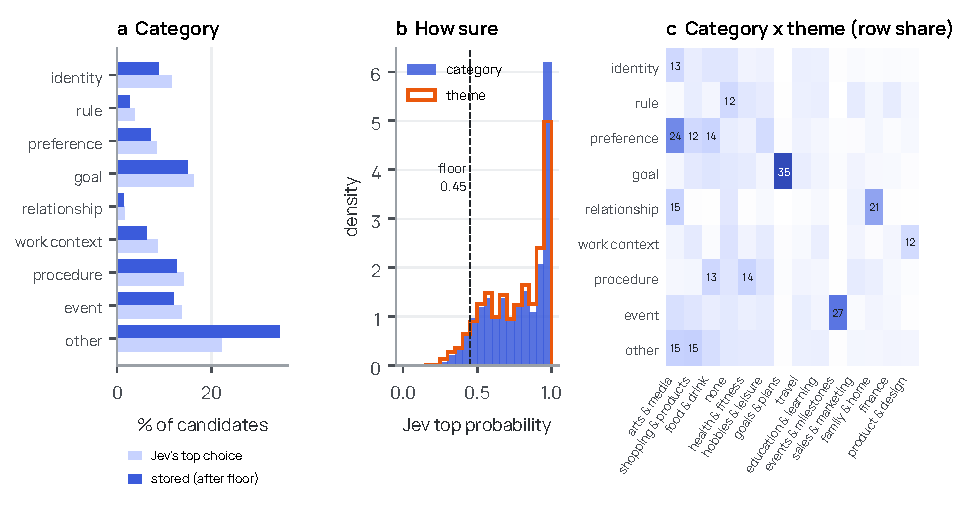
\includegraphics[width=\linewidth]{figures/fig_sort.pdf}
\caption{\textbf{How Jev sorted 85,013 candidate facts from the LongMemEval histories.} (a) Jev's top choice against
the stored category after the 0.45 floor; most of the difference is facts moved to ``other''. (b) Top-probability
distribution for category and theme. (c) Which themes each category's facts fell into (row share).}
\label{fig:sort}
\end{figure}

Figure~\ref{fig:sort} shows the classifier at work on the benchmark histories. The median top probability was 0.83
for category and 0.81 for theme. The heat map shows the two independent questions agreeing where they should: 35\% of goals fall in the
\emph{goals and plans} theme, 27\% of events in \emph{events and milestones}, 21\% of relationships in \emph{family and
home}, and preferences spread over arts and media, shopping, and food and drink, as one would expect from personal
chat. The ``none'' column holds facts whose best theme was below 0.45. 70 of
85,013 candidates (0.08\%) crossed the 0.5 injection flag; Section~\ref{sec:decisions} tests the check directly.

% ================================================================= 6
\section{Reconciliation: same, replaces, covers, related}\label{sec:reconcile}

\paragraph{Finding neighbours} For each candidate, memx runs vector search (10 hits) and full-text search (5 hits) over
the scope chain and over narrower scopes below it, and an exact lookup of the normalised text hash. Each neighbour falls
in a band by cosine similarity (Figure~\ref{fig:reconcile}): an identical hash is a duplicate; above 0.95 with no new
content words, the same negation polarity and the same numbers it is a duplicate without a model call (a
\emph{lexical guard}: ``likes coffee'' and ``does not like coffee'' embed as near-identical); between 0.45 and 0.95, or
above 0.95 with new words, Jev decides; below 0.45 it is unrelated. Up to five neighbours per direction go to Jev in one
request.

\paragraph{The verdict} Jev answers one Choice per neighbour with five options, worded as definitions
(Table~\ref{tab:verdicts}). Its context gives the neighbour's category, whether it lives in the same, a broader or a
narrower scope, and how the candidate's age compares (``the candidate is 3 weeks newer''). Floors are asymmetric:
``same'' needs 0.8, ``candidate replaces'' and ``neighbour covers'' need 0.9, the level above which Jev's destructive
verdicts agree with a larger model and are stable under option reordering (Section~\ref{sec:decisions}). Anything
below its floor becomes ``related'', which only links.

\paragraph{Guards} Three code rules hold back a ``replaces'' or ``covers'' at any probability, each logged with its
reason: the facts name different attributes in the extractor's \code{attribute} label (``page count'' vs ``reading
progress''); both came from the same extraction window (one statement split in two); or the candidate only describes
an earlier state (``the previous channel was \ldots'') and the neighbour does not. Held-back replacements are listed
on the insert receipt as \emph{possible replacements}.

\begin{table}[!htb]
\centering\small
\begin{tabularx}{\linewidth}{@{}l L L@{}}
\toprule
\thead{Verdict} & \thead{Definition given to Jev (abridged)} & \thead{Action}\\
\midrule
same & Both give the same information; the candidate adds nothing & reinforce the stored fact, drop the candidate\\ \rowrule
candidate replaces & They conflict, so both cannot be true now, and the candidate is newer; or it is a more specific version &
same scope: mark old \emph{replaced}; broader: \emph{shadow} it for this branch; narrower: retire it below\\ \rowrule
neighbour covers & The neighbour already says it more completely, or is the newer of two conflicting statements & store the candidate as history, already replaced\\ \rowrule
related & Same subject, both can be true & record a related link (used only to group output)\\ \rowrule
unrelated & Different subjects or attributes & nothing\\
\bottomrule
\end{tabularx}
\caption{\textbf{The five reconcile verdicts.} ``Neighbour covers'' lets a backfilled, older statement be stored as
history instead of overwriting the newer one.}
\label{tab:verdicts}
\end{table}

\begin{figure}[!htb]
\centering
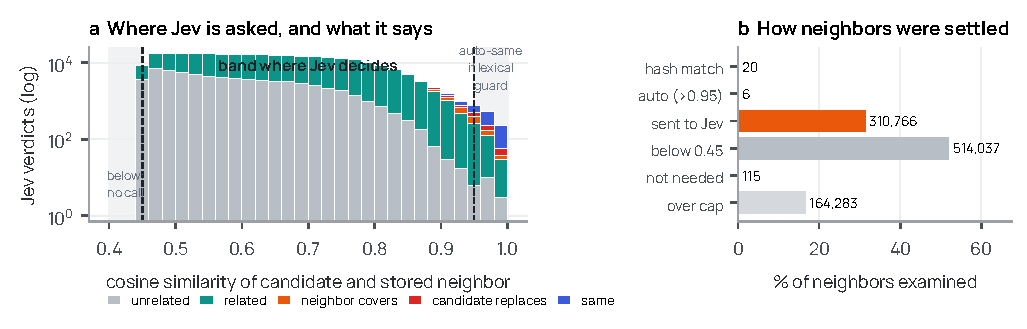
\includegraphics[width=\linewidth]{figures/fig_reconcile.pdf}
\caption{\textbf{Bands and verdicts on the benchmark data.} (a) Every Jev reconcile verdict by the cosine similarity of
the pair (log scale). The judge is asked only inside the 0.45--0.95 band; ``candidate replaces'' and ``same'' concentrate
at high similarity, but every verdict occurs across the band, which is why a threshold alone cannot decide. (b) How the
989,227 neighbours examined were settled: about half fell below the low band and never reached Jev.}
\label{fig:reconcile}
\end{figure}

\paragraph{Scopes} The verdict is turned into an action by where the neighbour lives (Figure~\ref{fig:scopes}).
Neighbours in the candidate's own scope or an ancestor decide whether the candidate is new at all. Neighbours in
narrower scopes, which will inherit the candidate, never block it: a newer broad fact retires outdated or duplicate
child facts, and anything else is linked. A narrow correction of a broad fact creates a \emph{shadow} link; the broad
fact stays active, and is hidden only from scopes whose chain contains the shadowing fact. Shadow and supersede links are
never walked during recall, so old versions cannot come back through the graph.

\begin{figure}[!htb]
\centering
\begin{tikzpicture}[
  font=\sffamily\scriptsize,
  sc/.style={draw=rule,fill=white,rounded corners=3pt,align=left,inner sep=3pt,text width=#1},
  sc/.default=3.6cm,
  arr/.style={-{Stealth[length=3pt]},draw=muted,line width=0.5pt},
  lev/.style={font=\sffamily\bfseries\scriptsize},
  fact/.style={font=\sffamily\scriptsize},
  ]
  \node[sc=4.0cm] (root) at (0,0) {\textbf{memory.acme}\\ F1: The on-call escalation channel is \#ops-alerts.};
  \node[sc=3.0cm] (alex) at (-2.1,-1.7) {\textbf{memory.acme.alex}\\ (no channel fact)};
  \node[sc=3.0cm,draw=shadowc] (sre) at (2.1,-1.7) {\textbf{memory.acme.sre}\\ F2: The SRE team's channel is now \#sre-pager.};
  \node[sc=3.0cm] (agent) at (-2.1,-3.2) {\textbf{memory.acme.alex.agent1}};
  \node[sc=3.0cm] (bot) at (2.1,-3.2) {\textbf{memory.acme.sre.}\textit{any child}};
  \draw[arr] (root) -- (alex); \draw[arr] (root) -- (sre); \draw[arr] (alex) -- (agent); \draw[arr] (sre) -- (bot);
  \draw[-{Stealth[length=4pt]},draw=shadowc,line width=0.9pt,dashed] (sre.east) to[bend right=40] node[right,pos=0.3,xshift=2mm,text=shadowc,align=left]{shadows F1\\ (replaces\\ at $\ge$0.9)} (root.east);
  \node[fact,below=1mm of agent,text width=3.0cm,align=left,text=pg] {sees F1 (\#ops-alerts)};
  \node[fact,below=1mm of bot,text width=3.0cm,align=left,text=shadowc] {sees F2; F1 hidden on this branch only};
  % right panel: broader correction retires below
  \node[sc=4.0cm] (r2) at (8.6,0) {\textbf{memory.acme.alex} (15 Oct)\\ F4: Alex does not want daily summaries.};
  \node[sc=4.0cm] (a2) at (8.6,-1.9) {\textbf{memory.acme.alex.agent1} (12 Sep)\\ \sout{F3: Send a daily summary at 9am.}};
  \draw[arr] (r2) -- (a2);
  \draw[-{Stealth[length=4pt]},draw=accent,line width=0.9pt] (r2.west) to[bend right=40] node[left,align=right,text=accent]{retires F3\\ below (Jev:\\ replaces, 0.98)} (a2.west);
  \node[fact,below=2mm of a2,text width=4.0cm,align=left] {A broader correction retires the outdated narrower fact;
  an older broad fact never retires a newer narrow one.};
  \draw[rule,line width=0.4pt] (5.35,0.6) -- (5.35,-3.9);
\end{tikzpicture}
\caption{\textbf{Corrections respect scope.} Left: a narrower scope's correction shadows the broader fact for its own
branch; siblings still see the original. Right: a broader correction retires a contradicting fact stored below it. The
verdict on the right is from the organisational probe (Section~\ref{sec:orgprobe}). On the left, Jev gave 0.89 in that
run, just under the 0.9 floor, so the two channel facts were linked instead; the SRE scope still answered correctly,
from the newer fact.}
\label{fig:scopes}
\end{figure}

% ================================================================= 7
\section{Relations: entity resolution with asymmetric priors}\label{sec:entities}

Entities (people, organisations, teams, systems, projects, places, products) connect facts without changing them. They
are keyed by tenant (the label under \code{memory}), so company-level and user-level facts in one tenant share them and
two tenants never do. Generic words (``the user'', ``the manager'') and lowercase descriptions (``the bakery down the
street'') are not entities; descriptive team names (``the data platform team'') are, because ownership questions route
through them.

For each name a candidate mentions, code finds up to three known entities it might be, and records \emph{why} each was
paired (Table~\ref{tab:pairing}). Code never merges two different spellings on its own, and Jev never has to search.
Full names and codes (``Marcus Oyelaran'', ``ARCHIVE-02''), and names already used earlier in the same insert, are
linked without asking. Each pairing reason gets its own question wording, with up to three facts about the known entity
as evidence, all in one request per candidate.

\begin{table}[!htb]
\centering\small
\begin{tabularx}{\linewidth}{@{}l l L l@{}}
\toprule
\thead{Pairing reason} & \thead{Example} & \thead{Found by} & \thead{Default}\\
\midrule
Identical name, ambiguous & ``Priya'' at work vs ``Priya'' from the bakery & same normalised name, single-word person or differing types & together\\ \rowrule
One name inside the other & ``Priya'' vs ``Priya Lindqvist'' & shared words & apart\\ \rowrule
Suggested alternative & ``Bangalore'' vs ``Blore'' & extractor-listed alternative names & apart\\ \rowrule
Similar name & ``Kubernetes'' vs ``K8s'' & name embeddings, cosine $\ge0.5$ & apart\\
\bottomrule
\end{tabularx}
\caption{\textbf{Why two names are compared, and which way the burden of proof runs.} ``Apart'' pairs merge only at
$P(\text{same})\ge0.7$; ``together'' pairs split only at $P(\text{different})\ge0.7$.}
\label{tab:pairing}
\end{table}

\paragraph{Why asymmetric} A wrong merge puts another person's facts into answers; a missed link costs one hop, so
different spellings start apart. Identical names start together: Jev's $P(\text{different})$ is high only when the
evidence really differs (``Priya from the bakery'' against Priya Lindqvist: 0.93). Each pairing reason has its own
question wording; asking whether a short name refers to a known entity, with facts about it, links ``Priya'' to
``Priya Lindqvist'' at 0.90 and keeps an unrelated Priya at 0.03. On a 20-pair probe set Jev got 18 right, and both
misses kept names apart, the safe direction. Embeddings only propose pairs: they find true variants but also
look-alikes (``Azure''/``AWS'' at 0.71).

\begin{figure}[!htb]
\centering
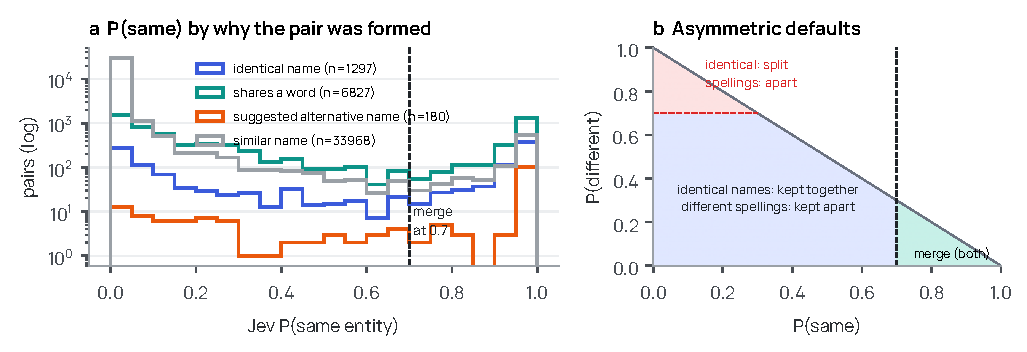
\includegraphics[width=\linewidth]{figures/fig_entities.pdf}
\caption{\textbf{Entity decisions on the benchmark data.} (a) Jev's $P(\text{same})$ for 42,272 name pairs by pairing
reason. Similar-embedding pairs are almost all judged different; extractor-suggested aliases almost all the same.
(b) The two decision rules over the probability simplex: different spellings merge only in the right band; identical
names are split only in the top-left corner.}
\label{fig:entities}
\end{figure}

A merged spelling is kept as an alias and the longer spelling becomes the display name. A repair pass
(\code{reresolve\_entities}) re-pairs stored entities by the same reasons and merges agreed pairs into the entity with
more facts.

% ================================================================= 8
\section{Retrieval: search, walk, grade, decay}\label{sec:recall}

\paragraph{Search} Vector search (40 hits) and full-text search (20 hits) over the visible facts, merged by reciprocal
rank fusion with $k=60$.

\paragraph{Walk} From the top 10 search hits (seeds, activation $a_s=\text{rrf}_s/\max\text{rrf}$), memx follows shared
entities for up to two hops. A fact $f$ reached from frontier fact $g$ through entity $e$ receives
\begin{equation}
\Delta a_f \;=\; a_g \cdot \frac{1}{\deg(e)-1}\cdot \delta,\qquad \delta=0.5\ \text{per hop},
\end{equation}
so activation is split evenly among the other facts naming $e$ and halved per hop; shared themes count at 30\% weight.
Entities named in more than 20\% of visible facts (and at least six), such as the company's own name, are \emph{hubs}
and are not walked. Each reached fact keeps its strongest path, preferring an all-entity path over a stronger one
through a theme, because ``via Marcus Oyelaran'' explains more than ``via career\_and\_role''. Up to eight facts the
search missed are added (Figure~\ref{fig:walk}).

\begin{figure}[!htb]
\centering
\begin{tikzpicture}[
  font=\sffamily\scriptsize,
  f/.style={draw=rule,fill=white,rounded corners=3pt,align=left,inner sep=3pt,text width=3.25cm},
  e/.style={draw=pg,fill=boxteal,rounded corners=7pt,inner sep=3pt,font=\sffamily\scriptsize\bfseries},
  hub/.style={draw=muted,fill=nac,rounded corners=7pt,inner sep=3pt,font=\sffamily\scriptsize,text=muted},
  q/.style={draw=jev,fill=boxorange,rounded corners=3pt,align=left,inner sep=3pt,text width=3.0cm},
  arr/.style={-{Stealth[length=3pt]},draw=ink,line width=0.55pt},
  w/.style={font=\sffamily\tiny,text=accent}]
  \node[q] (q) {\textbf{Query}\\ ``Can Alex run the ARCHIVE-02 schema migration on Friday?''};
  \node[f,right=6mm of q,draw=linkblue,line width=0.8pt] (f1) {\textbf{seed} (search rank 1)\\ Marcus Oyelaran approved retiring ARCHIVE-02. \hfill $a{=}1.0$};
  \node[e,right=6mm of f1] (marcus) {Marcus Oyelaran};
  \node[f,below=8mm of marcus] (f2) {\textbf{hop 1}\\ Marcus Oyelaran leads the data platform team. \hfill $a{=}0.25$};
  \node[e,left=6mm of f2] (dpt) {data platform team};
  \node[f,left=6mm of dpt] (f3) {\textbf{hop 2}\\ The data platform team owns all database migrations. \hfill $a{=}0.04$};
  \node[hub,above=4mm of marcus] (acme) {Acme Analytics (hub, cut)};
  \node[f,below=8mm of f3,xshift=0mm,text width=8.6cm,fill=titlebg,draw=jev] (g) {\textbf{Grade} (one Jev request): f3 is judged
  \emph{together with f2, through ``data platform team''}. Judged alone, ``owns all database migrations'' could look like
  background; with the bridge in view it is \emph{important}: the migration needs the data platform team's review.};
  \draw[arr] (q) -- (f1);
  \draw[arr] (f1) -- (marcus); \draw[arr] (marcus) -- node[w,right]{$\times\frac{1}{\deg-1}\times0.5$} (f2);
  \draw[arr] (f2) -- (dpt); \draw[arr] (dpt) -- (f3);
  \draw[draw=muted,dashed] (f1.north east) -- (acme.west);
  \draw[arr,draw=jev,dashed] (f3.south) -- (g.north -| f3.south);
\end{tikzpicture}
\caption{\textbf{The walk, and why linked facts are graded together.} Activation spreads from search hits through
non-hub entities and is halved per hop; each reached fact keeps its path, which is shown in the dashboard and passed to
the grader. The query and weights are illustrative.}
\label{fig:walk}
\end{figure}

\paragraph{Grade} One Jev request rates every candidate (up to 40 search hits plus walked facts) on a five-level Score:
irrelevant, background, useful, important, critical (relevance $=$ score$/4$). A walked fact is graded with its
instruction pointing at the fact it was reached from and the entity that links them, because a bridge fact
(``Priya Lindqvist leads the Security Team'') looks irrelevant to a question about Snowflake access when judged alone.
Search hits that also have a link are graded both alone and linked and keep the higher grade: a link may add
relevance, never remove it.

\paragraph{Cut, score and fit} Search hits need relevance $\ge0.3$; walked facts need $\ge0.5$. Survivors are scored
\begin{equation}
s(f) = r_f \cdot \bigl(0.6 + 0.4\, 2^{-\text{age}_f / h_{c(f)}}\bigr)\cdot\bigl(0.5+0.5\,\tau_f\bigr)\cdot
\min\bigl(1.3,\,1+0.05\ln(1+n_f)\bigr)\cdot \bigl(0.85 \text{ if walked}\bigr),
\end{equation}
where $h_c$ is the category half-life (Table~\ref{tab:cats}, Figure~\ref{fig:decay}), age counts from when the fact was
observed or last repeated, $\tau_f$ is the speaker's trust (user and named participants 1.0, documents 0.8 by default,
the assistant 0.6) and $n_f$ the number of times the fact has been recalled. Facts are taken in score order until the
budget or the 30-fact limit is reached, then rendered grouped by category in a fixed order, related facts nested,
events prefixed with their date. Scores choose which facts go in; they never change the order, so the same memory
always renders the same way.

\paragraph{History when asked} The grade request carries one extra yes/no question: does the query ask about an
earlier or changed state (``what was my previous goal?'')? If so, the versions each picked fact replaced are listed
under it, dated, within the budget. Related facts are always rendered with the date they were said, so two
disagreeing statements show which is newer.

\begin{figure}[!htb]
\centering
\begin{minipage}[t]{0.49\linewidth}\centering
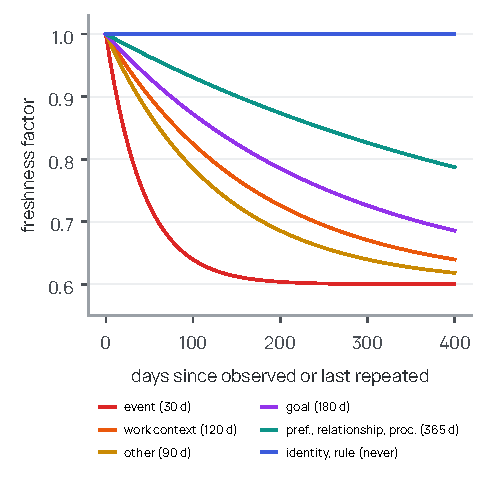
\includegraphics[width=\linewidth]{figures/fig_decay.pdf}
\caption{\textbf{Freshness factor by category.} Decay only ranks; it never hides a fact. Repeating a fact resets its
age.}\label{fig:decay}
\end{minipage}\hfill
\begin{minipage}[t]{0.49\linewidth}\centering
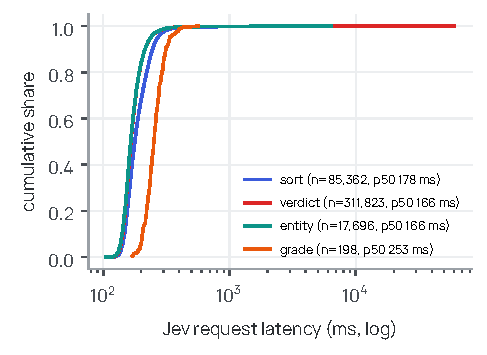
\includegraphics[width=\linewidth]{figures/fig_latency.pdf}
\caption{\textbf{Jev latency per request} across all logged decisions, by step (one request may carry many
questions).}\label{fig:latency}
\end{minipage}
\end{figure}

% ================================================================= 9
\section{Audit and explainability}\label{sec:audit}

Nothing is edited in place: replaced facts keep their row with \code{superseded\_by}, shadows are links, expiry is a
status change before a delayed purge. Every fact traces to its raw input and position, and to the decisions that
categorised and reconciled it. Ten tables hold the state; the \code{memx\_decision} table holds every Jev answer with its
full probability distribution, question version and latency, and doubles as the calibration dataset. Forgetting a
scope deletes its inputs, facts, links, entity mentions, decisions and recall logs in one transaction; the forget log
keeps counts and the requester, never content. The dashboard shows each insert's \emph{trace} (windows, candidates,
Jev's category and theme probabilities, entities found and merged, every neighbour on a similarity axis against the
bands, and the decision in plain words) and each recall's \emph{retrieval path}, including the walk and a table of every
candidate's ranks, grade, freshness, trust, score and reason.

\begin{tcolorbox}[enhanced,colback=titlebg,colframe=rule,arc=4pt,boxrule=0.4pt,left=6pt,right=6pt,top=4pt,bottom=4pt,
  title={\sffamily\footnotesize\bfseries An insert trace (abridged), from the organisational probe},coltitle=ink,colbacktitle=titlebg]
\footnotesize\ttfamily
said       "I don't want daily summaries anymore, please stop them."   (user, 2026-10-15, memory.acme.alex)\\
candidate  "The user does not want daily summaries."\\
sort       preference 0.99 | theme communication\_style | injection 0.07   (132 ms)\\
neighbour  "The user wants a daily summary of open tickets at 9am."  (memory.acme.alex.agent1, narrower)  sim 0.574\\
\hspace*{2em}verdict  candidate\_replaces 0.98 | neighbour\_covers 0.02 | others 0.00   (141 ms)\\
\hspace*{2em}guards   attributes compatible (preference/preference), different windows, present tense: pass\\
outcome    added; the agent-level fact retired below (row kept, superseded\_by set)
\end{tcolorbox}
